%\documentclass{beamer}
%\documentclass[draft]{beamer}
\documentclass[handout]{beamer}
%\documentclass[draft,handout]{beamer}

\usepackage[brazil]{babel}
\usepackage[latin1]{inputenc}
\usepackage[T1]{fontenc}
\usepackage{type1ec}
\usepackage{graphicx}
\usepackage{multirow}
\usepackage{soul}
\usepackage{ifpdf}

\ifpdf
	\usepackage{epstopdf}
\fi

%\let\newfloat=\undefined
\usepackage[boxed]{algorithm2e}
\usepackage{algorithmic}

%\newcommand{\theHalgorithm}{\arabic{algorithm}}

% Mudando o label dos algoritmos para portug�s
%\floatname{algorithm}{Algoritmo}

% Vari�veis matem�ticas
\newcommand{\C}{\mathcal{C}}
\newcommand{\Cl}{\mathcal{C}^{'}}
\newcommand{\D}{\mathcal{D}}
\newcommand{\Dl}{\mathcal{D}^{'}}
\newcommand{\Dlc}{\mathcal{D}^{'}_c}
\newcommand{\F}{\mathcal{F}}
\newcommand{\Fl}{\mathcal{F}^{'}}
\newcommand{\Flc}{\mathcal{F}^{'}_c}
\newcommand{\Fli}{\mathcal{F}^{'}_i}
\newcommand{\Flt}{\mathcal{F}^{'}_t}
\newcommand{\G}{\mathcal{G}}
\newcommand{\I}{\mathcal{I}}
\newcommand{\Il}{\mathcal{I}^{'}}
\newcommand{\M}{\mathcal{M}}
\newcommand{\Or}{\mathcal{O}}
\newcommand{\R}{\mathcal{R}}
%\newcommand{\Se}{\mathcal{S}}

\usetheme[compress]{Berlin}
%\usetheme{Berlin}

\title[Frequent and Orthogonal Patterns Mining]{Frequent and Orthogonal Patterns Mining and its Application in Associative Classification}
\author[Leandro S. Costa]{Leandro Souza Costa \\ Advisor: Wagner Meira Jr.}
\institute[DCC-UFMG]{Department of Computer Science \\ Federal University of Minas Gerais}
\logo{\includegraphics[height=.8cm]{../thesis/img/speed}}
\date[Master's Thesis]{Master's Thesis Defense \\ \today}

\begin{document}

\setbeamercovered{transparent}

\begin{frame}
\titlepage
\end{frame}

%\section*{Sum�rio}
%\begin{frame}[shrink=5]
%\tableofcontents
%\end{frame}

%\include{introducao_en}
%\include{classificacao_en}
%\section{Classifica��o Associativa}
\subsection{Contextualiza��o}

\begin{frame}{Modelos de Classifica��o}
	\begin{itemize}[<+-| alert@+>]
		\item Modelos propostos: redes neurais, estat�sticos, �rvores de decis�o, algoritmos gen�ticos, etc.;
		\item Modelo baseado em �rvores de decis�o � um dos mais indicados para Minera��o de Dados;
		\item Classifica��o Associativa produz resultados ainda melhores.
	\end{itemize}
\end{frame}

\subsection{Fundamentos Te�ricos}

\begin{frame}{Padr�es Freq�entes}
	\begin{itemize}[<+-| alert@+>]
%		\item Seja $\I$ um conjunto de itens;
		\item Um conjunto $X = \left\{i_1, \cdots, i_k\right\} \subseteq \I$, onde $\I$ � um conjunto de itens, � chamado de \textit{itemset} (ou padr�o);
		\item Uma transa��o sobre $\I$ � um par $T = \left(tid, I\right)$ onde $tid$ � o identificador da transa��o e $I$ � um \textit{itemset};
%		\item Dizemos que uma transa��o $T = \left(tid, I\right)$ � coberta por um \textit{itemset} $X \subseteq \I$, se $X \subseteq I$;
%	\end{itemize}
%\end{frame}
%
%\begin{frame}{Padr�es Freq�entes}
%	\begin{itemize}[<+-| alert@+>]
		\item Uma base de dados de transa��es $\D$ sobre $\I$ � um conjunto de transa��es sobre $\I$;
%		\item A freq��ncia de um \textit{itemset} $X$ em $\D$ � o n�mero de transa��es cobertas por $X$ em $\D$;
		\item O suporte de um \textit{itemset} $X$ em $\D$ � a probabilidade de $X$ ocorrer em uma transa��o $T \in \D$;
		\item Um padr�o � freq�ente se o seu suporte � maior ou igual a um dado valor relativo m�nimo $\sigma$, com $0 \leq \sigma \leq 1$.
	\end{itemize}
\end{frame}

\begin{frame}{Padr�es Freq�entes}
	\begin{block}{Defini��o}
		Seja $\D$ uma base de dados de transa��es sobre um conjunto de itens $\I$, e $\sigma$ um valor m�nimo de suporte. A cole��o de \textit{itemsets} freq�entes em $\D$ em rela��o a $\sigma$ � dado por: \[\F(\D,\sigma):=\left\{X \subseteq \I | suporte (X,\D) \geq \sigma \right\}.\]
	\end{block}
%	\pause
%	\begin{block}{Minera��o de Padr�es Freq�entes}
%		Dado um conjunto de itens $\I$, uma base de dados de transa��es $\D$ sobre $\I$, e um suporte m�nimo $\sigma$, encontre $\F(\D,\sigma)$.
%	\end{block}
\end{frame}

\begin{frame}{Regras de Associa��o}
	\begin{itemize}[<+-| alert@+>]
		\item Uma regra de associa��o � uma implica��o da forma $X \Rightarrow Y$, onde $X$ � um conjunto de itens em $\I$, e $Y$ � um �nico item em $\I$ que n�o est� presente em $X$;
%		\item A regra $X \Rightarrow Y$ � satisfeita no conjunto de transa��es $T$ com confian�a $0 \leq c \leq 1$ se, e somente se, pelo menos $c$\% das transa��es em $T$ que satisfazem $X$ tamb�m satisfazem $Y$;
%		\item O suporte de uma regra $X \Rightarrow Y$ em $\D$ � o suporte de $X \cup Y$ em $\D$, e a freq��ncia da regra � a freq��ncia de $X \cup Y$;
		\item O suporte de uma regra $X \Rightarrow Y$ em $\D$ � o suporte de $X \cup Y$ em $\D$;
		\item A regra $X \Rightarrow Y$ � satisfeita no conjunto de transa��es $T$ com confian�a $0 \leq \gamma \leq 1$ se, e somente se, a probabilidade condicional de encontrar $Y$ numa transa��o, dado que esta cont�m $X$, � maior que $\gamma$;
	\end{itemize}
\end{frame}
	
%\begin{frame}{Regras de Associa��o}
%	\begin{itemize}[<+-| alert@+>]
%		\item Dizemos que uma regra de associa��o � freq�ente se o seu suporte excede um determinado valor m�nimo $\sigma$;
%		\item A confian�a de uma regra de associa��o $X \Rightarrow Y$ em $\D$ � a probabilidade condicional de encontrar $Y$ numa transa��o, dado que esta cont�m $X$;
%		\item Dizemos que a regra � de confian�a se $P(Y|X)$ excede um determinado valor m�nimo de confian�a $\gamma$, com $0 \leq \gamma \leq 1$.
%	\end{itemize}
%\end{frame}

\begin{frame}{Regras de Associa��o}
	\begin{block}{Defini��o}
		Seja $\D$ uma base de dados de transa��es sobre um conjunto de itens $\I$, $\sigma$ um valor m�nimo para suporte e $\gamma$ um valor m�nimo para confian�a, o conjunto de regras de associa��o freq�entes e de confian�a considerando $\sigma$ e $\gamma$ � dado por:
		\begin{multline*}
			\R(\D,\sigma,\gamma) := \{X \Rightarrow Y|X,Y \subseteq \I, X \cap Y = \left\{ \right\}, X \cup Y \in \F(\D,\sigma), \\
			confianca(X \Rightarrow Y,\D) \geq \gamma\}.
		\end{multline*}
	\end{block}
\end{frame}

\begin{frame}{Classifica��o Associativa}
	\begin{itemize}[<+-| alert@+>]
		\item Dados de entrada: Cole��o de registros;
		\item Cada registro � caracterizado por um par $(x,y)$, onde $x$ � um conjunto de atributos comuns, e $y$ � um atributo especial, designado como \textbf{classe};
		\item Classifica��o � o processo de se descobrir uma fun��o $f$ que realiza o mapeamento de cada conjunto de atributos $x$ para uma das classes $y$ pr�-definidas.
	\end{itemize}
\end{frame}

\begin{frame}{Estrat�gias \textit{eager} e \textit{lazy}}
	\begin{block}{Estrat�gia \textit{eager}}
		Gera um conjunto de regras a partir da base de treinamento, e, para cada inst�ncia de teste, utiliza a melhor regra do conjunto para classific�-la.
	\end{block}
	\pause
	\begin{block}{Estrat�gia \textit{lazy}}
		Para cada inst�ncia de teste, gera um conjunto de regras a partir de uma proje��o da base de treinamento que possui apenas transa��es relacionadas com a inst�ncia de teste.
	\end{block}
\end{frame}

%\begin{frame}{LAC (\textit{Lazy Associative Classifier}}
%	\begin{itemize}[<+-| alert@+>]
%		\item Classificador associativo baseado na estrat�gia \textit{lazy}.
%	\end{itemize}
%\end{frame}

\subsection{M�tricas de Regras de Associa��o}

\begin{frame}{M�tricas Alternativas}
	\begin{itemize}[<+-| alert@+>]
		\item{Convic��o:} Definida como $conviccao(X \Rightarrow Y) = \frac{P(X) \times P(\neg Y)}{P(X \wedge \neg Y)}$, compara a probabilidade de $X$ aparecer sem $Y$ com a freq��ncia real do aparecimento de $X$ sem $Y$;
		\item{Leverage:} Definida como $leverage(X \Rightarrow Y) = P(X \wedge Y) - (P(X) \times P(Y))$, mede a diferen�a de $X$ e $Y$ aparecendo juntos na base de dados e o que seria esperado se $X$ e $Y$ fossem estatisticamente dependentes;
		\item{Lift:} Definida como $lift(X \Rightarrow Y) = \frac{P(X \wedge Y)}{P(X) \times P(Y)}$, mede quantas vezes $X$ e $Y$ ocorrem juntos a mais que o esperado se eles fossem estatisticamente independentes. Uma das desvantagens do \textit{lift} � ser suscept�vel a ru�dos em pequenas bases de dados;
	\end{itemize}
\end{frame}		

\begin{frame}{M�tricas Alternativas}
	\begin{itemize}[<+-| alert@+>]
		\item{Jaccard:} O coeficiente de Jaccard � uma medida estat�stica utilizada para comparar similaridade e diversidade entre conjuntos, definida pela raz�o entre a interse��o e a uni�o entre dois conjuntos. Esta m�trica � obtida pela express�o $jaccard(X \Rightarrow Y) = \frac{P(X \wedge Y)}{P(X)+P(Y)-P(X \wedge Y)}$;
		\item{Laplace:} Definida como $laplace(X \Rightarrow Y) = \frac{frequencia(X \wedge Y) + 1}{frequencia(X) + c}$, onde $c$ � o n�mero de classes do dom�nio;
		\item{Kulc:} Definida como $kulc(X \Rightarrow Y) = \frac{P(X \wedge Y)}{2}\left( \frac{1}{P(X)} + \frac{1}{P(Y)}\right)$, a medida \textit{Kulczynski} � muito utilizada na �rea qu�mica;
		\item{Cosseno:} Esta m�trica, bastante utilizada como medida de similaridade para textos,  � definida como $cosseno(X \Rightarrow Y) = \frac{P(X \wedge Y)}{\sqrt{P(X) \times P(Y)}}$;
	\end{itemize}
\end{frame}		

\begin{frame}{M�tricas Alternativas}
	\begin{itemize}[<+-| alert@+>]
		\item{Sensitividade:} Definida como $sensitividade(X \Rightarrow Y) = P(X|Y)$, sensitividade (ou \textit{recall}) � bastante utilizada em sistemas de recupera��o de informa��o;
		\item{Especificidade:} Definida como $especificidade(X \Rightarrow Y) = P(\neg Y | \neg X)$, esta m�trica representa a propor��o de verdadeiro-negativos sobre os casos negativos da regra.
	\end{itemize}
\end{frame}

\section{Frequent and Orthogonal Patterns}
\subsection{Contextualizing}

\begin{frame}{Frequent Patterns}
	\begin{itemize}[<+-| alert@+>]
		\item Widely used in several applications, including association rules, classification, clustering, indexing, etc.;
		\item Minimize the result is still a challenge:
		\begin{itemize}[<+-| alert@+>]
			\item One of the properties of Frequent Patterns is anti-monotonicity.
		\end{itemize}
		\item Minimize redundancy is another challenge:
		\begin{itemize}[<+-| alert@+>]
			\item There is limited work on finding those top-k patterns which demonstrate high-significance and low-redundancy simultaneously.
		\end{itemize}
	\end{itemize}
\end{frame}

\begin{frame}{Frequent Patterns}
	\begin{block}{Orthogonal Patterns}
		Our goal is to apply orthogonality in the frequent pattern mining problem, extracting a sub-set of patterns with high-significance and low-redundancy simultaneously.
	\end{block}
\end{frame}

\begin{frame}{Orthogonality Metrics}
	\begin{itemize}[<+-| alert@+>]
		\item It is necessary to define orthogonality metrics in order to evaluate sets;
		\item The Jaccard similarity coefficient complement applied to dataset coverage may be considered as an orthogonality metric applicable to two patterns: \[D(p_1,p_2) = 1 - \frac{|TS(p_1) \cap TS(p_2)|}{|TS(p_1) \cup TS(p_2)|},\] where $TS(p)$ is the set of transactions covered by $p$.
		\item We are interested in metrics applicable to sets of different sizes.
	\end{itemize}
\end{frame}

\subsection{Orthogonality Metrics}

\begin{frame}{Considering Pattern Structures}
	\begin{block}{Motivation}
		Two patterns are orthogonal if they don't share items. We say that the patterns $ABC$ and $DEF$ are orthogonal, but $ABC$ e $CDE$ are not, since the item $C$ is present in both patterns. This may be applied to bigger sets, for example, the patterns $AB$, $CD$ e $EF$ are orthogonal, but the patterns $AB$, $BC$ e $CD$ are not.
	\end{block}
\end{frame}
\begin{frame}{Considering Pattern Structures}
	\begin{itemize}[<+-| alert@+>]
		\item Let $\I$ be a set of items, $\D$ a dataset of transactions in $\I$, $\F$ the set of frequent patterns in $\D$, and $\Fl$ a sub-set of $\F$ ($\Fl \subseteq \F$);
		\item We say that $\Il \subseteq \I$ is the sub-set of items that appear in, at least, one of the patterns found in $\Fl$;
		\item For each item $i \subseteq \Il$ is given a weight: \[w_i = \frac{|\Fl|-|\Fli|}{|\Fl|-1},\] where $\Fli \subseteq \Fl$ is the sub-set of patterns from $\Fl$ that contains the item $i$;
	\end{itemize}
\end{frame}

\begin{frame}{Considering Pattern Structures}
	\begin{itemize}[<+-| alert@+>]
		\item The orthogonality based in patterns structure for the set is given by: \[O_e = \frac{\sum_{i \subseteq \Il} w_i}{|\Il|}.\]
	\end{itemize}
\end{frame}

\begin{frame}{Considering Transaction Coverage}
	\begin{block}{Motivation}
		Two patterns are orthogonal if they appear in different areas in dataset. In other words, if the sets of transactions covered by each pattern don't have elements in common.
	\end{block}
\end{frame}

\begin{frame}{Considering Transaction Coverage}
	\begin{figure}
	\centering
	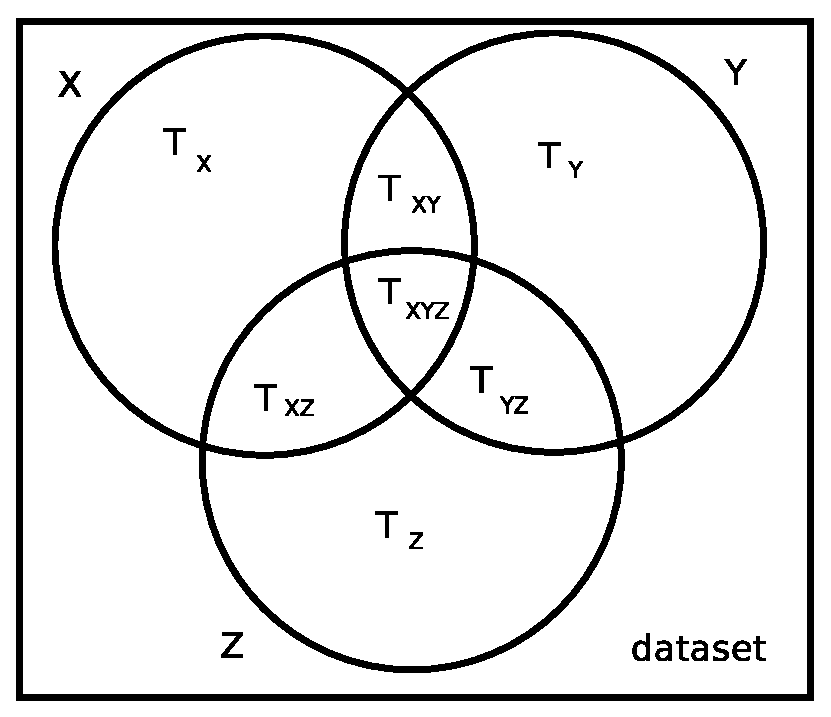
\includegraphics[width=0.5\textwidth]{../thesis/img/coverage}
	\caption{Visualization of Transaction Coverage in the Dataset}
	\label{fig:covex1}
	\end{figure}
\end{frame}

\begin{frame}{Considering Transaction Coverage}
	\begin{itemize}[<+-| alert@+>]
		\item Let $\I$ be a set of items, $\D$ a dataset of transactions in $\I$, $\F$ the set of frequent patterns in $\D$, and $\Fl$ a sub-set of $\F$ ($\Fl \subseteq \F$);
		\item We say that $\Dl \subseteq \D$ is the sub-set of transactions covered by, at least, one of the patterns found in $\Fl$;
		\item For each transaction $t \subseteq \Dl$ is given a weight: \[w_t = \frac{|\Fl| - |\Flt|}{|\Fl| - 1},\] where $\Flt$ is the sub-set of patterns from $\Fl$ that appear in the transaction $t$;
	\end{itemize}
\end{frame}

\begin{frame}{Considering Transaction Coverage}
	\begin{itemize}[<+-| alert@+>]
		\item The orthogonality based in transaction coverage is given by: \[O_t = \frac{\sum_{t \subseteq \Dl} w_t}{|\Dl|}.\]
	\end{itemize}
\end{frame}

\begin{frame}{Considering Class Coverage}
	\begin{block}{Motivation}
		Two patterns are orthogonal if they are found in transactions with distinct classes. In other words, the sets of transactions covered by the pattens may not have classes in common.
	\end{block}
\end{frame}

\begin{frame}{Considering Class Coverage}
	\begin{itemize}[<+-| alert@+>]
		\item Let $\I$ be a set of items, $\D$ a dataset of transactions in $\I$, $\F$ the set of frequent patterns in $\D$, $\Fl$ a sub-set from $\F$ ($\Fl \subseteq \F$) and $\Dl \subseteq \D$ the sub-set of transactions covered by, at least, one of the patters found in $\Fl$;
		\item We say that $\C$ is the set of classes associated to transactions in $\D$ and $\Cl \subseteq \C$ the sub-set of classes associated to transactions in $\Dl$;
		\item For each class $c \subseteq \Cl$ is given a weight: \[w_c = \frac{|\Fl| - |\Flc|}{|\Fl| - 1},\] where  $\Flc$ is the sub-set of patterns from $\Fl$ that cover a number of transactions with class $c \subseteq \Cl$ higher than $90\%$ of the expected average;		
	\end{itemize}
\end{frame}

%\begin{frame}{Considerando Cobertura de Classes}
%	\begin{itemize}[<+-| alert@+>]
%		\item Para cada classe $c \subseteq \Cl$ � dado um peso: \[w_c = \frac{|\Fl| - |\Flc|}{|\Fl| - 1},\] onde $\Flc$ � o sub-conjunto de padr�es de $\Fl$ que cobrem uma quantidade de transa��es de classe $c \subseteq \Cl$ maior que $90\%$ da m�dia esperada;
%	\end{itemize}
%\end{frame}

\begin{frame}{Considering Class Coverage}
	\begin{itemize}[<+-| alert@+>]
		\item The orthogonality based in class coverage is given by: \[O_c = \frac{\sum_{c \subseteq \Cl} w_c}{|\Cl|}.\]
	\end{itemize}
\end{frame}

\subsection{Associative Classification and Orthogonality}

\begin{frame}{Using Orthogonality in LAC}
	\begin{itemize}[<+-| alert@+>]
		\item For each test instance, LAC (\textit{Lazy Associative Classifier}) builds a projection of training dataset with only transactions that share items with the instance;
		\item After that, the algorithm gets a set of frequent patterns according to a support given by the user;
		\item With these patterns, it generate association rules used to classify the instance.
	\end{itemize}
\end{frame}

\begin{frame}{Using Orthogonality in LAC}
	\begin{itemize}[<+-| alert@+>]
		\item In this work, orthogonality was used to extract, from the frequent patterns set, a sub-set of orthogonal patterns;
		\item The association rules were generated from this sub-set.
	\end{itemize}
\end{frame}

\begin{frame}{Heuristic to Get Orthogonal Sets}
	\begin{itemize}[<+-| alert@+>]
		\item Find the sub-set of patterns with best orthogonality metric is NP-Hard;
		\item It was developed a greedy heuristic that starts with an orthogonal set with two elements, and, iteratively, tries to obtain a new set with one more element adding candidate patterns and modifying the set in order to maximize the metric.
	\end{itemize}
\end{frame}

\begin{frame}[shrink=5]{Heuristic to Get Orthogonal Sets}
%\begin{frame}{Heur�stica de Obten��o de Conjuntos Ortogonais}

\begin{algorithm}[H]
\caption{OLAC}
\label{alg:olac}
\begin{algorithmic}[1]

\REQUIRE $\D, \sigma$
	\STATE $\F \leftarrow FindFrequentPatterns (\D, \sigma)$
	\STATE $Sort (\F)$
	\STATE $\Or \leftarrow GetFirstAvailablePattern (\F)$
	\REPEAT
		\STATE $rate \leftarrow GetOrthogonalityRate (\Or)$
%		\STATE $\Or_{try} \leftarrow \Or \cup GetFirstAvailablePattern (\F)$
%		\STATE $rate_{try} = GetOrthogonalityRate (\Or_{try})$
%		\FOR {$P \in \F, P \notin \Or_{try}$}
%			\STATE $S \leftarrow GetMoreSimilar (\Or, P)$
%			\STATE $\Or_{try} \leftarrow \Or_{try} \cup P \ \backslash \ S$
%			\STATE $rate_{tmp} = GetRate (\Or)$
%			\IF {$rate_{tmp} \leq rate_{try}$}
%				\STATE $\Or_{try} \leftarrow \Or_{try} \cup S \  \backslash \  P$
%			\ELSE
%				\STATE $rate_{try} \leftarrow rate_{tmp}$
%			\ENDIF
%		\ENDFOR
		\STATE $\Or_{c} \leftarrow GetNextCandidateSet (\Or, \F)$
		\STATE $rate_{c} = GetOrthogonalityRate (\Or_{c})$
		\IF {$rate_{c} \geq rate$}
			\STATE $\Or \leftarrow \Or_{c}$
		\ENDIF
	\UNTIL {$rate_{c} < rate$}
	\STATE $\R \leftarrow \Or$

\end{algorithmic}
\end{algorithm}

\end{frame}

\begin{frame}[shrink=5]{Heuristic to Get Orthogonal Sets}
%\begin{frame}{Heur�stica de Obten��o de Conjuntos Ortogonais}

\begin{algorithm}[H]
\caption{OLAC - GetNextCandidateSet}
\label{alg:olac_getNextCandidateSet}
\begin{algorithmic}[1]

\REQUIRE $\Or, \F$
\STATE $\Or_{c} \leftarrow \Or \cup GetFirstAvailablePattern (\F)$
\STATE $rate_{c} = GetOrthogonalityRate (\Or_{c})$
\FOR {$P \in \F, P \notin \Or_{c}$}
	\STATE $S \leftarrow GetMoreSimilar (\Or_{c}, P)$
	\STATE $\Or_{c} \leftarrow \Or_{c} \cup P \ \backslash \ S$
	\STATE $rate_{try} = GetRate (\Or_{c})$
	\IF {$rate_{try} > rate_{c}$}
		\STATE $rate_{c} \leftarrow rate_{try}$
	\ELSE
		\STATE $\Or_{c} \leftarrow \Or_{c} \cup S \  \backslash \  P$
	\ENDIF
\ENDFOR
\RETURN $\Or_{c}$
%
\end{algorithmic}
\end{algorithm}

\end{frame}

\subsection{The ORIGAMI Strategy}

\begin{frame}{Contextualizing}
The \textbf{ORIGAMI} is a graph mining algorithm found in literature, where the authors introduce a definition for $\alpha$-orthogonality and $\beta$-representativity, and present a new paradigm for mining a summary representation of the set of frequent graphs by considering the distances in the pattern space.
\end{frame}

\begin{frame}{$\alpha$-orthogonality Definition}
	\begin{itemize}[<+-| alert@+>]
		\item Let $\F$ be the set of all frequent sub-graphs of a collection;
		\item Let $sim : \F \times \F \rightarrow \left[0, 1\right]$ be a symmetric binary function that returns the \textit{similarity} between two graphs;
		\item Given a collection of graphs $\G$, and an upper-bound for similarity $\alpha \in \left[0, 1\right]$, we say that the sub-set of graphs $\R \subseteq \G$ is \textbf{$\alpha$-orthogonal} with respect to $\G$ if, and only if, for any $G_a, G_b \in \R, sim(G_a, G_b) \leq \alpha$ and for any $G_i \in \G \backslash \R$ there exists a $G_j \in \R, sim(G_i, G_j) > \alpha$;
	\end{itemize}
\end{frame}

\begin{frame}{$\alpha$-orthogonality Definition}
	\begin{itemize}[<+-| alert@+>]
		\item Given a collection of graphs $\G$, an $\alpha$-orthogonal set $\R \subseteq \G$ and a lower-bound for similarity $\beta \in \left[0, 1\right]$, we say that $\R$ \textbf{represents} a graph $G \in \G$ if there exists some $G_a \in \R$ such that $sim(G_a, G) \geq \beta$. Given $\Upsilon(\R,\G) = \left\{G \in \G : \exists G_a \in \R, sim(G, G_a) \geq \beta\right\}$, we say that $\R$ is a $\beta$-representative set for $\Upsilon(\R, \G)$;
	\end{itemize}
\end{frame}

\begin{frame}{$\alpha$-orthogonality Definition}
	\begin{itemize}[<+-| alert@+>]
		\item Given a collection of graphs $\G$, an $\alpha$-orthogonal set and its $\beta$-representative set $\R$, we call \textbf{residue} of $\R$ the set of patterns not represented in $\G$, given as $\Delta(\R, \G) = \G \backslash \left\{ \R \cup \Upsilon(\R, \G) \right\}$, the \textit{residue} of $\R$ is defined as the cardinality of its residue-set $|\Delta(\R, \G)|$. Finaly, we define the average residue similarity for $\R$ as follows: $ars(\R, \G) = \frac{\sum_{G_b \in \Delta(\R, \G)} {max_{G_a \in \R} \left\{sim(G_a, G_b)\right\}}}{|\Delta(\R, \G)|}$.
	\end{itemize}
\end{frame}

\begin{frame}{$\alpha$-orthogonality Definition}
	\begin{block}{Objective}
		The goal is to find sets of $\alpha$-orthogonal and $\beta$-representative graphs related to the maximal sub-graphs set $\M$.
	\end{block}
\end{frame}

\begin{frame}{The ORIGAMI Algorithm}

\begin{algorithm}[H]
\caption{ORIGAMI}
\label{alg:origami}
\begin{algorithmic}[1]

\REQUIRE $\D, \sigma, \alpha, \beta$
\STATE $EM \leftarrow EdgeMap (\D)$
\STATE $\F_1 \leftarrow FindFrequentEdges (\D, \sigma)$
\STATE $\widehat{\M} \leftarrow 0$
\WHILE {$\neg StopCondition ()$}
	\STATE $M \leftarrow RandomMaximalGraph (\D, \F_1, EM, \sigma)$
	\STATE $\widehat{\M} \leftarrow \widehat{\M} \cup M$
\ENDWHILE
\STATE $\R \leftarrow OrthogonalRepresentativeSets (\widehat{\M}, \alpha, \beta)$

\end{algorithmic}
\end{algorithm}

\end{frame}

\begin{frame}{The ORIGAMI Adaptation}
	\begin{itemize}[<+-| alert@+>]
		\item It was implemented an adaptation of ORIGAMI for the Associative Classification Problem;
		\item It was implemented a heuristic to get maximal patterns based on the article;
		\item It was implemented a heuristic to get orthogonal patterns based on the article.
	\end{itemize}
\end{frame}

\begin{frame}{Heuristic to Get Maximal Patterns}
	\begin{itemize}[<+-| alert@+>]
		\item The algorithm starts with an empty result-set;
		\item On each iteration, it tries to get the largest frequent pattern possible, selection items randomly;
			\begin{itemize}[<+-| alert@+>]
				\item If the algorithm chooses an item that is already in the pattern, or that makes the pattern infrequent, a counter is decremented;
				\item The stop-condition for the candidate pattern generation is that the number of wrong chooses for the random item should be, at most, equal to the test instance size.
			\end{itemize}
	\end{itemize}
\end{frame}

\begin{frame}{Heuristic to Get Maximal Patterns}
	\begin{itemize}[<+-| alert@+>]
		\item After generate a new maximal pattern, the algorithm tries to insert it in the result-set;
		\begin{itemize}[<+-| alert@+>]
			\item If the pattern is already in the set, the algorithm decrements a second counter of tries;
			\item The stop condition for the maximal patterns set generation is that number of candidate patterns generated that are not maximal or are already in the set should be, at most, equal to the test instance size.
		\end{itemize}
	\end{itemize}
\end{frame}

\begin{frame}{Heuristic to Get the Orthogonal Patterns Set}
	\begin{itemize}[<+-| alert@+>]
		\item The algorithm starts with a residue equal to $0$ (zero);
		\item On each iteration, it tries to get a new orthogonal set selecting, randomly, maximal patterns found in the first step of the algorithm, and adding them to the result-set;
		\begin{itemize}[<+-| alert@+>]
			\item If the algorithm selects a pattern that is already in the set or does not have similarity lower than $\alpha$ with all the other patterns of the set, the algorithm decrements a counter of tries;
			\item The stop-condition is that the maximum number of wrong patterns chosen should be, at most, equal to the number of maximal patterns.
		\end{itemize}
	\end{itemize}
\end{frame}

\begin{frame}{Heuristic to Get the Orthogonal Patterns Set}
	\begin{itemize}[<+-| alert@+>]
		\item After generate a new orthogonal set, the algorithm calculate its residue-value;
		\item If the residue is the best until now, it consider the set found as the new best result;
		\item The stop-condition for the algorithm is that the maximum number of orthogonal sets generated that don't improve the result should be, at most, equal to the number of maximal patterns.
	\end{itemize}
\end{frame}


%\begin{frame}{Heur�stica de Obten��o de Conjuntos Ortogonais}
%	\begin{itemize}[<+-| alert@+>]
%		\item No in�cio do algoritmo, o conjunto-solu��o � inicializado com apenas um elemento, e a m�trica de ortogonalidade do conjunto com o valor $0$ (zero), e ent�o come�a o ciclo de itera��es:
%		\begin{enumerate}[<+-| alert@+>]
%			\item Um novo elemento � inclu�do ao conjunto;
%			\item � realizada uma busca por todo o conjunto de padr�es que n�o fazem parte do conjunto-solu��o. Durante este procedimento, cada padr�o verificado � inclu�do na solu��o, substituindo, neste conjunto, o elemento que mais se assemelha �quele. Se a m�trica de ortogonalidade do conjunto melhorou, o algoritmo mant�m a troca. Se n�o, a troca � desfeita, e o pr�ximo padr�o da seq��ncia � verificado;
%			\item Ao final do processo, o algoritmo compara a m�trica de ortogonalidade obtida com a m�trica do conjunto anterior (que possu�a um elemento a menos). Se a m�trica se manteve, ou melhorou, o algoritmo mant�m o novo conjunto como solu��o, e volta ao in�cio do ciclo. Se n�o, o algoritmo termina o ciclo, e o conjunto anterior � dado como resultado.
%		\end{enumerate}
%	\end{itemize}
%\end{frame}


% M�tricas de Ortogonalidade
% Classifica��o Associativa e Ortogonalidade
% Estrat�gia ORIGAMI

%\include{ortogonalidade_v2_en}
\section{Evaluation}
\subsection{Experiments}

\begin{frame}{The Applicative \textbf{olac}}
	\begin{itemize}[<+-| alert@+>]
		\item In the applicative \textbf{olac} we have the implementation of three different approaches of an association rules based classifier:
		\begin{itemize}[<+-| alert@+>]
			\item The LAC (\textit{Lazy Associative Classifier}) approach, that is the \textit{lazy} strategy in his original version(and non-orthogonal);
			\item The OLAC (\textit{Orthogonal Lazy Associative Classifier}) approach, that is a variant of the \textit{lazy} strategy considering orthogonality;
			\item The ORIGAMI, that is the adaptation presented for the ORIGAMI strategy.
		\end{itemize}
	\end{itemize}
\end{frame}

%\begin{frame}[fragile,shrink=30]{Op��es de Execu��o}
%
%\begin{verbatim}
%Usage: ./olac [options]
%Options:
%  -i, --training-file       Set the training file
%  -t, --testing-file        Set the testing file
%  -s, --support             Set the support
%  -c, --confidence          Set the confidence
%  -r, --run-mode            Set the run mode [c,o] [CLASSICAL, ORTHOGONAL]
%  -p, --pattern-set         Set the pattern set type [f,m,r] [FREQUENT, MAXIMAL,
%                              RANDOM MAXIMAL]
%  -n, --min-num-rules       Set the minimum number of rules generated
%  -l, --max-num-rank-rules  Set the maximum number of rules considered (rank size)
%  -m, --min-rule-len        Set the minimum length of the rules
%  -x, --max-rule-len        Set the maximum length of the rules
%  -o, --orth-mode           Set the orthogonality mode [h,p,o] [HEURISTICAL,
%                              POLYNOMIAL, ORIGAMI]
%\end{verbatim}
%
%\end{frame}

%\begin{frame}[fragile,shrink=30]{Op��es de Execu��o}
%
%\begin{verbatim}
%  -e, --orth-metric         Set the orthogonality metric [s,c,l,a] [STRUCTURE,
%                              TRANSACTION COVERAGE, CLASS COVERAGE, ALL]
%  -w, --orth-method         Set the way metrics are used [s,p,a] [SET, PAIR AVERAGE,
%                              ALL]
%  -g, --orth-pat-ordering   Set the way patterns are ordered for heuristic
%                              [s,r,i,z,n] [SORTED, REVERSE SORTED, SORTED BY SIZE,
%                              REVERSE SORTED BY SIZE, NONE]
%  -u, --rule-measure        Set the rule measure used [s,c,j,k,o,n,e,p,l,i,v]
%                              [SUPPORT, CONFIDENCE, JACCARD, KULC, COSINE,
%                              CONVICTION, SENSITIVITY, SPECIFICITY, LAPLACE,
%                              LIFT, LEVERAGE]
%  -a, --origami-alpha       Set the alpha parameter used by ORIGAMI
%  -b, --origami-beta        Set the beta parameter used by ORIGAMI
%  -d, --debug               Set the level of debug [-1,0,1,2,3,4] [SILENT, NO DEBUG,
%                              LOW LEVEL, MEDIUM LEVL, HIGH LEVEL, MAX LEVEL]
%  -v, --verbose             Use verbose mode
%  -h, --help                Display this information
%\end{verbatim}
%
%\end{frame}

%\subsection{Experimentos}

\begin{frame}{Methodology}
	\begin{itemize}[<+-| alert@+>]
		\item We used 26 datasets from \textbf{UCI} (\textit{UC Irvine Machine Learning Repository});
		\item We used 10-fold cross-validation and the final results of each experiment represent the average of the ten runs.
			\end{itemize}
\end{frame}

%\begin{frame}{Metodologia}
%	\begin{itemize}[<+-| alert@+>]
%		\item Como resultados foram considerados a m�dia das dez execu��es diferentes para cada base de dados;
%		\item Os par�metros utilizados nos testes se encontram na tabela \ref{tab:table_test_parms_presentation};
%		\item Todas as combina��es poss�veis destes par�metros foram realizadas, com exce��o da combina��o tamanho m�ximo de regra  $1$ e m�trica de ortogonalidade $s$ para o OLAC.
%	\end{itemize}
%\end{frame}

\begin{frame}[shrink]{Methodology}
	\begin{centering}
	\begin{table}[htbp]
	\centering
		\resizebox{0.95\textwidth}{!} {
		\begin{tabular}{|l|c|}
		\hline
		\textbf{Parameters}	& \textbf{Values}	\\
		\hline
		support			& $\left\{ 0.0001, 0.001, 0.01, 0.1, 0.2, 0.3, 0.4, 0.5, 0.6, 0.7, 0.8, 0.9, 0.95, 0.99, 1 \right\}$	\\
		\hline
		confidence		& $\left\{ 0.0001, 0.001, 0.01, 0.1, 0.2, 0.3, 0.4, 0.5, 0.6, 0.7, 0.8, 0.9, 0.95, 0.99, 1 \right\}$				\\
		\hline
		min-num-rules		& $\left\{ 1 \right\}$				\\
		\hline
		max-num-rank-rules	& $\left\{ 1,10,100,1000,10000,100000,1000000 \right\}$		\\
		\hline
		min-rule-len		& $\left\{ 1 \right\}$				\\
		\hline
		max-rule-len		& $\left\{ 1,2,3 \right\}$		\\
		\hline
		rule-measure		& $\left\{ s,c,j,k,o,n,e,p,l,i,v \right\}$	\\
		\hline
		orth-metric		& $\left\{ e,c,l,a \right\}$			\\
		\hline
		orth-method		& $\left\{ s,p \right\}$				\\
		\hline
		orth-pat-ordering	& $\left\{ s,r,i,z,n \right\}$			\\
		\hline
		origami-alpha		& $\left\{ 0.1,0.2,0.3,0.4,0.5,0.6,0.7,0.8,0.9 \right\}$		\\
		\hline
		origami-beta		& $\left\{ 0.1,0.2,0.3,0.4,0.5,0.6,0.7,0.8,0.9 \right\}$		\\
		\hline
		\end{tabular}
		}
	\caption{Parameters Used for All Approaches}
	\label{tab:table_test_parms}
\end{table}

	\end{centering}
\end{frame}

\begin{frame}[shrink]{Better Results for Each Dataset}
	\begin{centering}
	\includegraphics[width=\textwidth]{../thesis/graphs/histogram_best_run_for_each_db_acc_en}
	\end{centering}
\end{frame}

\begin{frame}[shrink]{Better Results for Each Dataset}
	\begin{centering}
	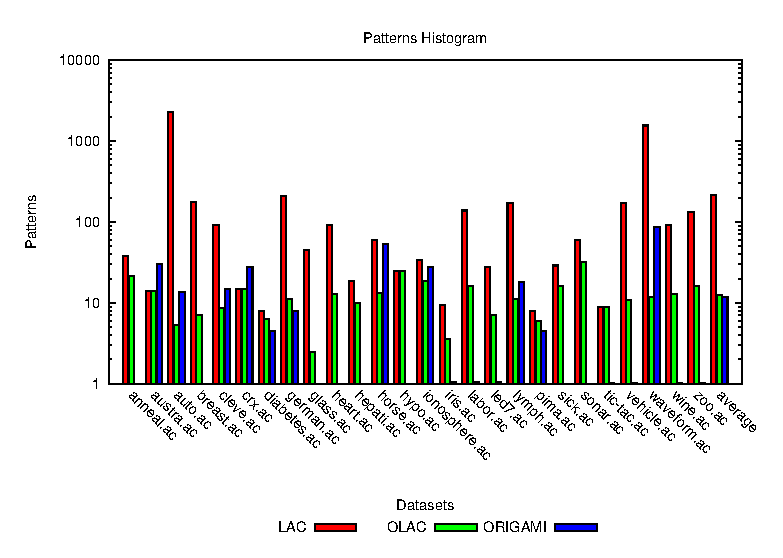
\includegraphics[width=\textwidth]{../thesis/graphs/histogram_best_run_for_each_db_pat_en}
	\end{centering}
\end{frame}

\begin{frame}[shrink]{Better Results for Each Dataset}
	\begin{centering}
	\includegraphics[width=\textwidth]{../thesis/graphs/histogram_best_run_for_each_db_rul_en}
	\end{centering}
\end{frame}

\begin{frame}[shrink]{Better Results in Average for All Datasets}
	\begin{centering}
	\includegraphics[width=\textwidth]{../thesis/graphs/histogram_best_run_for_avg_db_acc_en}
	\end{centering}
\end{frame}

\begin{frame}[shrink]{Better Results in Average for All Datasets}
	\begin{centering}
	\includegraphics[width=\textwidth]{../thesis/graphs/histogram_best_run_for_avg_db_pat_en}
	\end{centering}
\end{frame}

\begin{frame}[shrink]{Better Results in Average for All Datasets}
	\begin{centering}
	\includegraphics[width=\textwidth]{../thesis/graphs/histogram_best_run_for_avg_db_rul_en}
	\end{centering}
\end{frame}

\begin{frame}[shrink]{Execution Parameters}
	\begin{centering}
	\input{../thesis/tables/table_best_parms_for_avg_db_en.tex}
	\end{centering}
\end{frame}

\begin{frame}
	\begin{block}{Results obtained with LAC using the best parameters for OLAC}
		Patterns: $249.03$ \\
		Rules: $628.12$ \\
		Accuracy: $0.54$
	\end{block}
\end{frame}

\begin{frame}[shrink]{Comparing the Results}
	\begin{centering}
	\begin{table}[htbp]
	\centering
%		\resizebox{0.95\textwidth}{!} {
		\begin{tabular}{|l|c|c|c|c|}
		\hline
				& \textbf{OLAC}		& \textbf{OLAC}			& \textbf{$\neg$ OLAC}	& \textbf{$\neg$ OLAC}	\\
		\textbf{Datasets}	& \textbf{\&}		& \textbf{\&}			& \textbf{\&}			& \textbf{\&}			\\
				& \textbf{LAC}		& \textbf{$\neg$ LAC}		& \textbf{LAC}			& \textbf{$\neg$ LAC}		\\
		\hline
		anneal.ac       & 95.11         & 1.13               & 0.75                     & 3.01                          \\
		\hline
		austra.ac       & 84.93         & 1.88               & 1.45                     & 11.74                         \\
		\hline
		auto.ac         & 39.51         & 6.83               & 4.39                     & 49.27                         \\
		\hline
		breast.ac       & 96.28         & 0.29               & 1.00                     & 2.43                          \\
		\hline
		cleve.ac        & 81.19         & 1.32               & 1.98                     & 15.51                         \\
		\hline
		crx.ac          & 84.93         & 1.59               & 1.88                     & 11.59                         \\
		\hline
%		diabetes.ac     & 76.82         & 1.04               & 1.30                     & 20.83                         \\
%		\hline
%		german.ac       & 70.40         & 3.40               & 3.10                     & 23.10                         \\
%		\hline
%		glass.ac        & 63.08         & 4.21               & 1.40                     & 31.31                         \\
%		\hline
%		heart.ac        & 82.96         & 0.37               & 1.48                     & 15.19                         \\
%		\hline
%		hepati.ac       & 85.16         & 1.94               & 0.00                     & 12.90                         \\
%		\hline
%		horse.ac        & 70.38         & 3.53               & 3.26                     & 22.83                         \\
%		\hline
%		hypo.ac         & 97.94         & 0.06               & 0.09                     & 1.90                          \\
%		\hline
%		ionosphere.ac   & 90.03         & 1.14               & 2.56                     & 6.27                          \\
%		\hline
%		iris.ac         & 94.00         & 0.67               & 0.67                     & 4.67                          \\
%		\hline
%		labor.ac        & 89.47         & 1.75               & 3.51                     & 5.26                          \\
%		\hline
%		led7.ac         & 61.72         & 4.31               & 4.97                     & 29.00                         \\
%		\hline
%		lymph.ac        & 79.73         & 2.70               & 0.68                     & 16.89                         \\
%		\hline
%		pima.ac         & 76.82         & 0.52               & 1.04                     & 21.61                         \\
%		\hline
%		sick.ac         & 97.04         & 0.04               & 0.18                     & 2.75                          \\
%		\hline
%		sonar.ac        & 80.29         & 2.40               & 2.88                     & 14.42                         \\
%		\hline
%		tic-tac.ac      & 56.47         & 6.78               & 3.86                     & 32.88                         \\
%		\hline
%		vehicle.ac      & 56.86         & 6.50               & 2.72                     & 33.92                         \\
%		\hline
%		waveform.ac     & 71.12         & 6.74               & 1.54                     & 20.60                         \\
%		\hline
		$\vdots$        & $\vdots$      & $\vdots$           & $\vdots$                 & $\vdots$                      \\
		\hline
		wine.ac         & 96.07         & 0.00               & 2.81                     & 1.12                          \\
		\hline
		zoo.ac          & 73.27         & 0.99               & 0.00                     & 25.74                         \\
		\hline
		average         & 78.91         & 2.39               & 1.90                     & 16.80                         \\
		\hline
		\end{tabular}
%		}
	\caption{Comparison between LAC and OLAC (number of correct and wrong classifications)}
	\label{tab:comparison_lac_olac}
\end{table}

	\end{centering}
\end{frame}

% O Aplicativo olac
% Exemplo de Execu��o
% Experimentos

\section{Conclusions}
\subsection{Results}

\begin{frame}{Accuracy}
	\begin{itemize}[<+-| alert@+>]
		\item With orthogonality based approaches we got good results, very close to the classical approach one:
		\begin{itemize}[<+-| alert@+>]
			\item Considering the best parameters for each dataset, the values for accuracies obtained by LAC, OLAC and ORIGAMI were, respectively, $0.843$, $0.840$ e $ 0.839$;
			\item Considering the best parameters for the average of the results, the values for accuracy obtained by LAC, OLAC and ORIGAMI were, respectively, $0.808$, $0.813$ e $0.782$.
		\end{itemize}
	\end{itemize}
\end{frame}

\begin{frame}{Patterns}
	\begin{itemize}[<+-| alert@+>]
		\item The number of patterns used to generate the rules by the orthogonal approaches were lower than by the classical approach:
		\begin{itemize}[<+-| alert@+>]
			\item Considering the best parameters for each dataset, the number of patters used by LAC, OLAC and ORIGAMI were, respectively, $213$, $12$ e $12$;
			\item Considering the best parameters for the average of the results, the number of patterns used by LAC, OLAC and ORIGAMI were, respectively, $19$, $12$ e $1$.
		\end{itemize}
	\end{itemize}
\end{frame}

\begin{frame}{Rules}
	\begin{itemize}[<+-| alert@+>]
		\item The number of rules generated by the orthogonal approaches were much lower than by the classical approach:
		\begin{itemize}[<+-| alert@+>]
			\item Considering the best parameters for each dataset, the number of rules generated by LAC, OLAC and ORIGAMI were, respectively, $628$, $25$ e $23$;
			\item Considering the best parameters for the average of the results, the number of rules generated by LAC, OLAC and ORIGAMI were, respectively, $51$, $31$ e $1$.
		\end{itemize}
	\end{itemize}
\end{frame}

\begin{frame}{Other Results}
	\begin{itemize}[<+-| alert@+>]
		\item The orthogonality metric based in pattern structure obtained the best results;
		\item The association rule metrics that obtained the best results were conviction by LAC and OLAC and confidence by ORIGAMI;
		\item Most of fails found in classification based in orthogonality was not caused by the low orthogonality metric. They were found because sometimes, the different patterns used, induced the results to the wrong class.
	\end{itemize}
\end{frame}

\subsection{Future Works}

\begin{frame}{Next Steps}
	\begin{itemize}[<+-| alert@+>]
		\item Use orthogonality in another points of a classification algorithm;
		\item Research for new heuristics of orthogonal patterns extraction, in order to improve performance;
		\item Research for new algorithms of frequent pattern mining that consider  orthogonality while generating the frequent patterns;
		\item Use of a hybrid approach OLAC-ORIGAMI.
	\end{itemize}
\end{frame}

\subsection{End}
\begin{frame}[c]
\begin{center}
\Large
\alert {Questions?}
\Large
\end{center}
\end{frame}


\end{document}
